\documentclass[journal]{IEEEtran}

%\usepackage[retainorgcmds]{IEEEtrantools}
%\usepackage{bibentry}
\usepackage{xcolor,soul,framed} %,caption

\colorlet{shadecolor}{yellow}
% \usepackage{color,soul}
\usepackage[pdftex]{graphicx}
\graphicspath{{../pdf/}{../jpeg/}}
\DeclareGraphicsExtensions{.pdf,.jpeg,.png}

\usepackage[cmex10]{amsmath}
%Mathabx do not work on ScribTex => Removed
%\usepackage{mathabx}
\usepackage{array}
\usepackage{mdwmath}
\usepackage{mdwtab}
\usepackage{eqparbox}
\usepackage{url}


% ----------------------------------------------

% Definitions of languages: ------------
\usepackage{listings}
\lstdefinestyle{cStyle}{
  basicstyle=\scriptsize,
  breakatwhitespace=false,
  breaklines=true,
  captionpos=b,
  keepspaces=true,
  numbersep=5pt,
  showspaces=false,
  gobble=4,
  tabsize=4,
  showstringspaces=false,
  showtabs=false,
}
\renewcommand*{\lstlistingname}{Code}

% ----------------------------------------------




% \hyphenation{op-tical net-works semi-conduc-tor}

%\bstctlcite{IEEE:BSTcontrol}


%=== TITLE & AUTHORS ====================================================================
\begin{document}
\bstctlcite{IEEEexample:BSTcontrol}
    \title{Reinforcement Learning}
  \author{Carlos~Matheus~Barros~da~Silva,
  ~\IEEEmembership{Computer Engineering Bachelor Student of ITA}
  \\Prof. Marcos~Ricardo~Omena~de~Albuquerque~Máximo}

% The paper headers
\markboth{INSTITUTO TECNOLÓGICO DE AERONÁUTICA, May~2019
}{Reinforcement Learning}

% ====================================================================
\maketitle


% === ABSTRACT ==============================================================
% ============================================================================
\begin{abstract}

This paper evaluates two \textit{Temporal Difference Learning} techniques, \textit{SARSA} and \textit{Q-Learning}.

Both techniques have been implemented and passed by some tests. On the end It was avaliated the learning with a car that needs to follow a track.

It was observed that both implementation worked as expected. The \textit{Q-Learning} having a faster learning, converging to a local maximum with much less iteration than the \textit{SARSA} algorithm.

% === KEYWORDS ===============================================================
% ============================================================================
\begin{IEEEkeywords}
    Temporal Difference Learning, SARSA, Q-Learning, Reinforcement Learning
\end{IEEEkeywords}
\end{abstract}

\IEEEpeerreviewmaketitle

% ====================================================================
% ====================================================================
% ====================================================================


% === I. INTRODUCTION ========================================================
% =============================================================================
\section{Introduction}

\IEEEPARstart{R}{e}inforcement learning (RL) is an area of machine learning concerned with how software agents ought to take actions in an environment so as to maximize some notion of cumulative reward. Reinforcement learning is one of three basic machine learning paradigms, alongside supervised learning and unsupervised learning.

It differs from supervised learning in that labelled input/output pairs need not be presented, and sub-optimal actions need not be explicitly corrected. Instead the focus is finding a balance between exploration (of uncharted territory) and exploitation (of current knowledge).

The environment is typically formulated as a Markov decision process (MDP), as many reinforcement learning algorithms for this context utilize dynamic programming techniques. The main difference between the classical dynamic programming methods and reinforcement learning algorithms is that the latter do not assume knowledge of an exact mathematical model of the MDP and they target large MDPs where exact methods become infeasible.

Temporal difference (TD) learning refers to a class of model-free reinforcement learning methods which learn by bootstrapping from the current estimate of the value function. These methods sample from the environment, like Monte Carlo methods, and perform updates based on current estimates, like dynamic programming methods.

While Monte Carlo methods only adjust their estimates once the final outcome is known, TD methods adjust predictions to match later, more accurate, predictions about the future before the final outcome is known. This is a form of bootstrapping, as illustrated with the following example:

''Suppose you wish to predict the weather for Saturday, and you have some model that predicts Saturday's weather, given the weather of each day in the week. In the standard case, you would wait until Saturday and then adjust all your models. However, when it is, for example, Friday, you should have a pretty good idea of what the weather would be on Saturday – and thus be able to change, say, Saturday's model before Saturday arrives.``

Temporal difference methods are related to the temporal difference model of animal learning.

% ==========================================================================
\section{Algorithms Implementation}
% \section{Neural Network Implementation}

Both Techniques implementation can be seen on the file \textit{reinforcement\_learning}. The essence of the implementation can be seen on the Code \ref{code:rl}.

% The implementation was based on the file \textit{lenet5}. The essence of the implementation can be seen on the Code \ref{code:lenet}

\lstinputlisting[
    language=python,
    caption={Code of both \textit{Temporal Difference Learning} techniques: \textit{SARSA} and \textit{Q-Learning}},
    label={coderl},
    style=cStyle,
    firstline=4,
    lastline=163
]{./../code/reinforcement_learning.py}
% \lstinputlisting[
%     language=python,
%     caption={Code of Convolutional Neural Network \textit{lenet5}},
%     label={code:lenet},
%     style=cStyle,
%     firstline=5,
%     lastline=83
% ]{./../code/lenet5.py}

\section{Temporal Difference Techniques Analysis}

\subsection{Initial test Analysis}

\subsubsection{SARSA}

In order to initially evalute \textit{SARSA} technique, it was run the file \textit{test\_rl.py} setted to test \textit{SARSA}.

With this setup it was obtained the output represented on the Code \ref{code:sarsa}.

\lstinputlisting[
    language=python,
    caption={Output of \textit{SARSA} test, It is denoted the Action-value Table and the Greedy policy learnt},
    label={code:sarsa},
    style=cStyle,
]{./../code/results_sarsa/test_result.txt}

In this test was observed a slow converge of \textit{SARSA} in a way that running this same test multiple times might result um some Greedy policy slightly differents.

\subsubsection{Q-Learning}

In order to initially evaluate \textit{Q-Learning} technique, it was run the file \textit{test\_rl.py} setted to test \textit{Q-Learning}.

With this setup it was obtained the output represented on the Code \ref{code:qlearning}.

\lstinputlisting[
    language=python,
    caption={Output of \textit{Q-Learning} test, It is denoted the Action-value Table and the Greedy policy learnt},
    label={code:qlearning},
    style=cStyle,
]{./../code/results_q_learning/test_result.txt}

In this test was observed a faster converge of \textit{Q-Learning} technique, in a way that it is less frequent than \textit{SARSA} to get a variation on the Greedy policy by the end of the test.

It was observed as well that the \textit{Q-Learning} algorithm is, as well, slightly faster than the \textit{SARSA}, in a way that more iterations are completed in \textit{Q-Learning} in a given time.

\subsection{LeNet-5 Convolutional Neural Network Analysis}

On Image \ref{img:classification_one} and \ref{img:classification_two} it is possible to see two examples of correctly classified test cases.

% \begin{figure}
%   \begin{center}
%   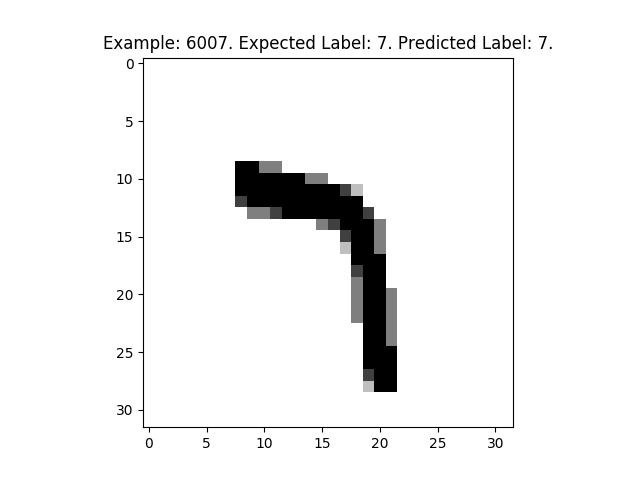
\includegraphics[width=2.8in]{./../code/test_image_6007.png}
%   \caption{Example of a correctly classified test case, was expected 7 and was predicted as 7.}
%   \label{img:classification_one}
%   \end{center}
% \end{figure}
%
% \begin{figure}
%   \begin{center}
%   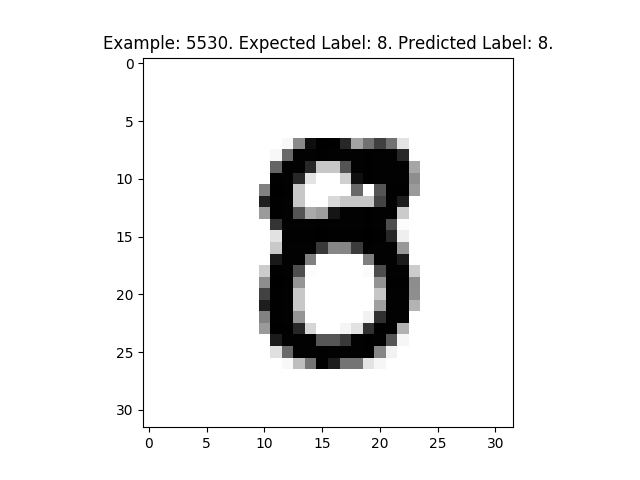
\includegraphics[width=2.8in]{./../code/test_image_5530.png}
%   \caption{Example of a misclassified test case, was expected 8 and was predicted as 8.}
%   \label{img:classification_two}
%   \end{center}
% \end{figure}

% \lstinputlisting[
%     language=python,
%     caption={Output for \textit{evaluate lenet5}},
%     label={code:eval_lenet5_out},
%     style=cStyle,
% ]{./../code/output.txt}

As said before, in 1.3\% of the test cases ware misclassified. In Image \ref{img:misclassification_one} and Image \ref{img:misclassification_two} is possible to see two examples of test cases of misclassification.

% \begin{figure}
%   \begin{center}
%   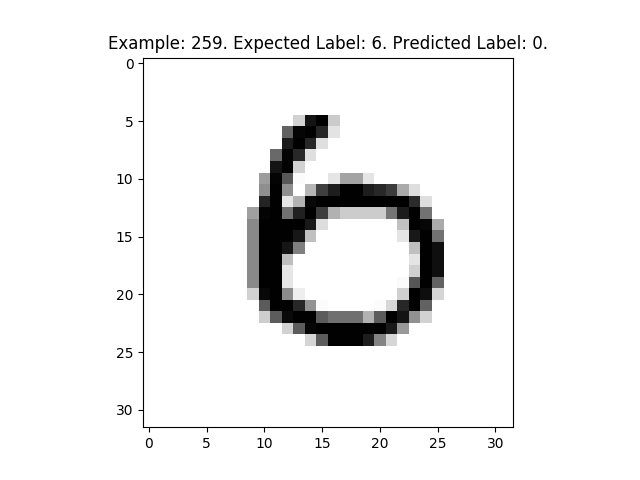
\includegraphics[width=2.8in]{./../code/misclassified_image_259.png}
%   \caption{Example of a misclassified test case, was expected 6 and was predicted as 0.}
%   \label{img:misclassification_one}
%   \end{center}
% \end{figure}
%
% \begin{figure}
%   \begin{center}
%   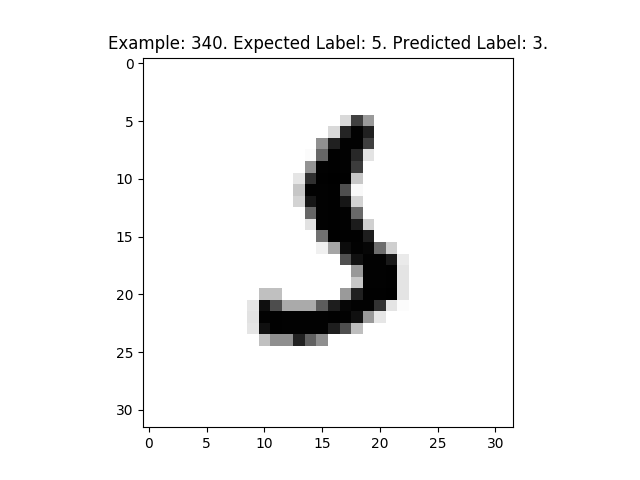
\includegraphics[width=2.8in]{./../code/misclassified_image_340.png}
%   \caption{Example of a misclassified test case, was expected 5 and was predicted as 3.}
%   \label{img:misclassification_two}
%   \end{center}
% \end{figure}

\subsection{LeNet-5 Convolutional Neural Network Analysis on TensorBoard}

In \textit{Tensor Board} it was possible to see that occured a fast decrase on loss function and a rapidly accuracy to converge in more than 98\% of acuracy. On Image \ref{img:accuracy} and Image \ref{img:loss_func} it is possible to see the graphs representing the converge of \textit{accuracy} and \textit{loss function} respectively.

% \begin{figure}
%   \begin{center}
%   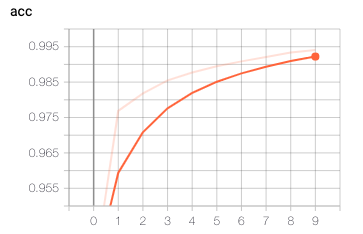
\includegraphics[width=2.8in]{./../code/tensorboard/tensor_board_accuracy_graph.png}
%   \caption{Accuracy Graph generated by TensorBoard}
%   \label{img:accuracy}
%   \end{center}
% \end{figure}
%
% \begin{figure}
%   \begin{center}
%   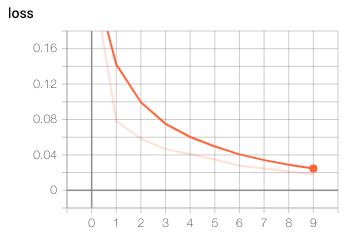
\includegraphics[width=2.8in]{./../code/tensorboard/tensor_board_loss_graph.png}
%   \caption{Loss Function Graph generated by TensorBoard}
%   \label{img:loss_func}
%   \end{center}
% \end{figure}

TensorBoard also provided an overview of the Neural Network format, this is denoted on Image \ref{img:tensorboard_main} and Image \ref{img:tensorboard_aux}.

% \begin{figure}
%   \begin{center}
%   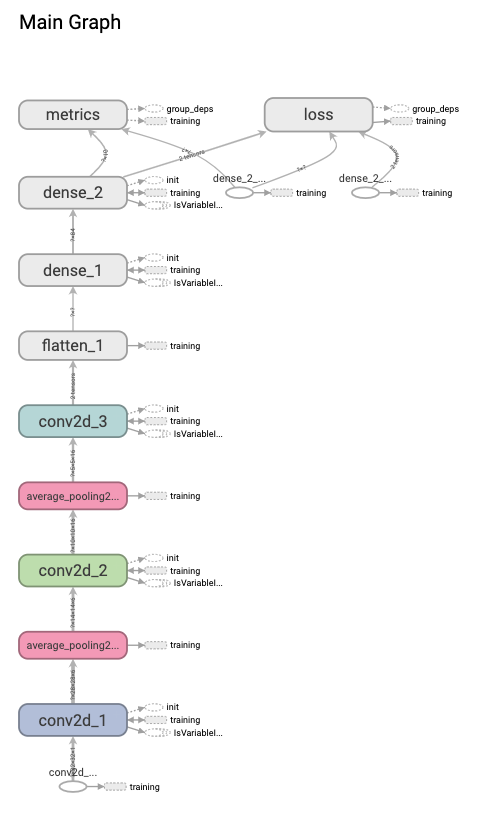
\includegraphics[width=2.8in]{./../code/tensorboard/tensor_board_main_graph.png}
%   \caption{TensorBoard Main Graph.}
%   \label{img:tensorboard_main}
%   \end{center}
% \end{figure}
%
% \begin{figure}
%   \begin{center}
%   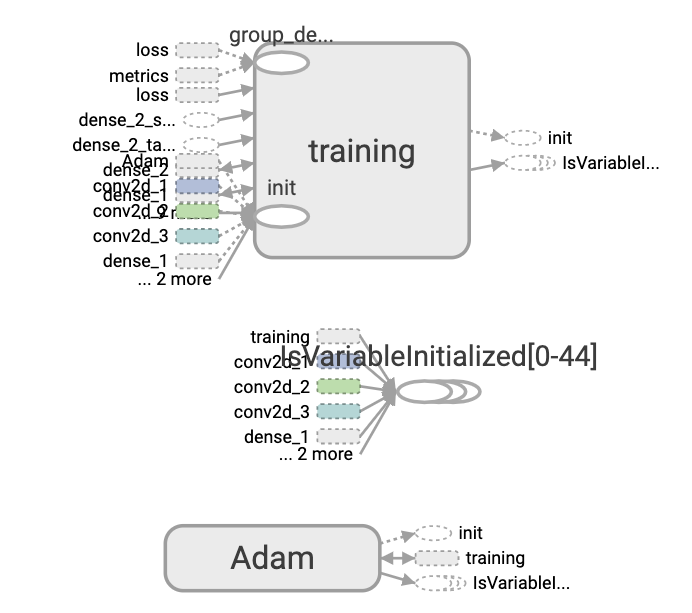
\includegraphics[width=2.8in]{./../code/tensorboard/tensor_board_auxiliary_nodes.png}
%   \caption{TensorBoard Auxiliary Nodes.}
%   \label{img:tensorboard_aux}
%   \end{center}
% \end{figure}

\section {Conclusion}

It was clear, therefore, that the Convolutional Neural Network worked as expected. The number prediction was very accurate having 98.7\% of accuracy on the data set.

\vfill
\end{document}
